\chapter{Dataset Generation}
\section{Workload Sampling}
We first generate sample workloads based on the application-provided query templates T. We create N random sample workloads, each containing m queries. Here, N and m must be sufficiently large so that query interaction patterns emerge and the decision tree model can be properly trained. However, m must also be sufficiently small so that for each sample workload we can identify the optimal schedule in a timely manner. 

In order to ensure that our sampling covers the space of possible workloads, we rely on uniform direct sampling of the query templates. If the sampling is not uniform, the decision tree may not be able to learn how two query templates interact, or the decision tree may have very little information about certain templates. Furthermore, we generate a large number of samples in order to ensure that our workload samples will also include workloads that are imbalanced with respect to the number of unique templates they include. This allows us to handle skewed workloads.

\section{Optimal Schedule Generation}
Given a set of sample workloads, we train a model based on the optimal schedules for these workloads. To produce these optimal solutions, we represent schedules as paths on a weighted graph, and we find the minimum cost path on this graph. This graph-based approach\cite{marcus2016wisedb} provides a number of advantages. First, each “best” path represents not only an optimal schedule, but also the steps taken to reach that optimal schedule. The information relevant to each optimal decision is captured by each vertex’s state. Second, a graph representation lends itself to a natural way of eliminating redundancy in the search space via careful, strategic path pruning. Finally, the well-studied nature of shortest-path problems enables the application of deeply-understood algorithms with desirable properties.
\subsection{Graph Construction}
Given a sample workload \(Q = \{q^x_1 , q^y_2 , ...\}\), we construct a directed, weighted graph G(V, E) where vertices represent intermediate steps in schedule generation, i.e., partial schedules and a set of remaining queries to be scheduled. Edges represent actions, such as renting a new VM or assigning a query to a VM. The cost (weight) of each edge will be the cost of performing a particular action (e.g., the cost of starting a new VM). We refer to this as a scheduling graph. Formally, each vertex v ∈ V has a schedule for some queries of the workload, \(v_s = \{vm^i_1, vm^k_2, ...\}\), which includes the VMs to be rented for these queries. Each VM j of type i, \(vm^i_j\), is a queue of queries that will be processed on that VM, \(vm^i_j = [q^x_k , q^y_m, ...]\). Hence, vs represents possible (potentially partial) schedules for the workload Q. Each \(v\) also has a set of unassigned queries from Q, \(v_u\), that must still be placed onto VMs. 

The start vertex, \(A \in V\) , represents the initial state where all queries are unassigned. Therefore, \(A_u\) includes all the queries in the given workload and \(A_s\) is empty. If a vertex \(g \in V\) has no unassigned queries, we say that vertex g is a goal vertex and its schedule \(g_s\) is a complete schedule.
\begin{figure}
\centering
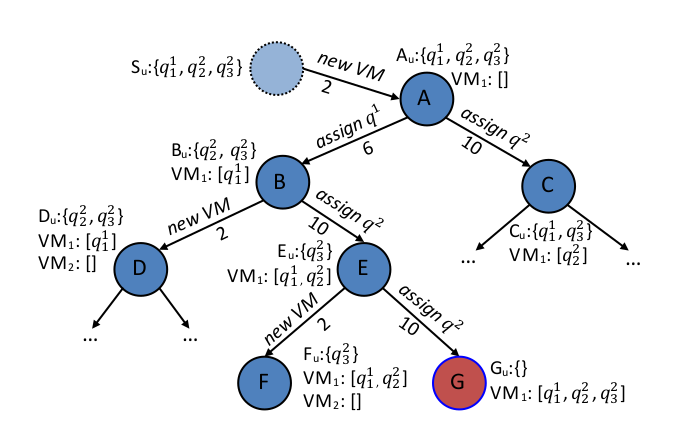
\includegraphics[width=1.0\textwidth]{scheduling_graph.png}
\caption{\label{fig:scheduling_graph}A subgraph of a scheduling graph for two query templates and \(Q = \{q^1_1, q^2_2, q^3_2\}\)}
\end{figure}

An edge in E represents one of two possible actions:
\begin{enumerate}
\item A start-up edge \((u, v, i)\) represents renting a new VM of type \(i, vm^i_j\) . It connects a vertex u to v where v has an additional empty VM, i.e., \(v_s = u_s \bigcup vm^i_j\). It does not assign any queries, so \(u_u = v_u\). The weight of a start-up edge is the cost to provision a new VM of type \(i: w(u, v) = f^i_s\). 

\item A placement edge \((u, v, q^x_y)\) represents placing an unassigned query \(q^x_y \in u_u\) into the queue of a rented VM in vs. It follows that \(v_u = u_u-q^x_y\) . Because our system is agnostic to the specifics of any particular query, the placement of an instance of query template \(T_x\) is equivalent to placing any other instance of \(T_x\). Therefore, we include only a single placement edge per query template even if the template appears more than once in \(u_u\). The cost of an edge that places query \(q^x_y\) into a VM of type i is the execution time of the query multiplied by the cost per unit time of the VM, plus any additionally incurred penalties:
\begin{equation} \label{penalty}
w(u, v) = [l(q^x_y, i)\times f^i_r ]+[p(R, v_s) - p(R, u_s)]
\end{equation}
\end{enumerate}
\subsection{Graph Reduction}
To improve the runtime of the search algorithm, we reduce the graph in a number of ways. First, we include a start-up edge only if the last VM provisioned has some queries assigned to it, i.e., we allow renting a new VM only if the most recently provisioned VM is not empty. Second, queries are assigned only to the most recently provisioned VM, i.e., each vertex has outgoing placement edges that assign a query only to the most recently added VM. This reduces the number of redundant paths in the graph. This reduction can be applied without loss of optimality, e.g. without eliminating any goal vertices.
\subsection{Search Algorithm}
We searched for the minimum cost path from the start vertex to a goal vertex using the A* search algorithm \cite{hart1968formal} which offers a number of advantages. First, it is complete, meaning that it always finds an optimal solution if one exists. Second, A* \cite{hart1968formal} can take advantage of an admissible heuristic, h(v), to find the optimal path faster. An admissible h(v) provides an estimate of the cost from a vertex v to the optimal goal vertex that is always less or equal to the actual cost, i.e., it must never overestimate the cost. For any given admissible heuristic, A* \cite{hart1968formal} is optimally efficient, i.e., no other complete search algorithm could search fewer vertices with the same heuristic. 
\subsubsection{Heuristic function}
We define a heuristic function h(v) \cite{hart1968formal} that calculates the cheapest possible runtime for the queries that are still unassigned at v. In other words, h(v) sums up the cost of the cheapest way to process each remaining query by assuming VMs could be created for free:\\
\begin{equation} \label{heuristic}
h(v) = \sum _{q^x_y \in v_u} min_i (f^i_r \times l(q^x_y , i))
\end{equation}
\section{Feature Extraction}
After the generation of the optimal schedules for each of the sampled workloads, we generated the training set for our decision tree classifier. The training set consists of (decision, features) pairs indicating the decisions that was made by A* while calculating optimal schedules and performance/workload related features at the time of the decision. Each decision represents an edge in the search graph, and is therefore a decision to either
(a) create a new VM of type i, or
(b) assign a query of template \(T_j\) to the most recently created VM. 

We map each decision (edge) (u, v) in the optimal path to a set of features of its origin vertex u since there is a correspondence between a vertex and the optimal decision made at that vertex. Specifically, for a given vertex u, the edge selected in the optimal path is independent of u’s parents or children but depends on the unassigned queries \(u_u\) and the schedule so far, \(u_s\). Hence, we extract features from each of the vertices in all the optimal paths we collected for all the sample workloads.
\subsection{Feature Selection}
Features should be:
\begin{enumerate}
\item Agnostic to the specifics of the query templates and performance goals. This will allow our framework to be customizable and enable it to learn good strategies independently of the query templates and performance metric expressed by the application.
\item Effective features must be unrelated to the size of the workload, since the large workload sizes encountered at runtime will not be represented in the training sample workloads, whose size is restricted in order to obtain the optimal schedules in a timely manner.
\item Features must be independent from one another to avoid extracting redundant information.
\end{enumerate}
Based on the above, we extracted the following features for each vertex v along the optimal path:
\begin{enumerate}
\item \textbf{Wait-time:} The amount of time that a query would have to wait before being processed if it were placed on the most recently created VM. Formally, wait-time is equal to the execution time of all the queries already assigned to the last VM. This feature can help our model decide which queries should be placed on the last added VM based on their deadline. For example, if a machine’s wait time has exceeded the deadline of a query template, it is likely that no more queries of this template should be assigned to that VM. Alternatively, if a machine’s wait time is very high, it is likely that only short queries should be assigned.
\item \textbf{Proportion-of-template-X:} Proportion-of-template-X is the ratio between the number queries of template X assigned to the VM and the total number of queries assigned to the VM. For example, if the VM currently has four queries assigned to it, with one of those queries being of template T1 and three being of template T2, then we extract the features proportion-of-T1=0.25 and proportion-of-T2=0.75. We only need to consider the most recently created VM because the assignment edges in the reduced graph only assign queries to the most recent VM. Since each sample workload contains only a limited number of queries, keeping track of the exact number of instances of each query template would not scale to large workloads. Therefore, we track the proportion instead.
\item \textbf{Cost-of-template-X:} The cost incurred (including any penalties) by placing a query of template X on the most recently created VM. cost-of-X is equal to the weight of the outgoing assignment edge for template X. This allows our model to check the cost of placing an instance of a certain query template and, based on its value, decide whether to assign another query to the last rented VM or create a new VM.
\item \textbf{Have-template-X}: Whether or not a query of template X is still unassigned. This feature helps our model understand how the templates of the unassigned queries affects the decisions on the optimal path. If there is no instance of some query template \(T_j\) unassigned, then the model places one of the remaining templates. If an instance of \(T_j\) exists, the model might prefer to schedule that as opposed to any other template.

\item \textbf{Supports-template-X:} whether or not the most recently created VM is capable of processing a query of class X. This feature is needed when not all VM types are capable of handling every type of query. It is used in Multiple VM-type systems.
\end {enumerate}
The extraction of these features in Optimal Schedules along with the decision it chooses generates the training set for the learning model. So, the training set is basically a set of \((f,d)\) instances where f is the features chosen and d is the respective decision taken.

We note that while these features are not enough to uniquely identify a vertex and thus learn the exact conditions that lead to the optimal schedule, they can shed light on the workload/performance conditions related to the optimal decision. Furthermore, although we cannot claim that these features will always allow our system to learn effective heuristics, our experimental results indicate that these features allow to learn a reasonable cross-section
of the scheduling algorithm space, and that they are expressive enough to generate scheduling strategies capable of efficiently handling commonly used performance goals
